
%%%%%%%%%%%%%%%%%%%%%%%%%%%%%%%%%%%%%%%%%%%%%%%%%%%%%%%%%%%%%%%%%%%%%%%%%%%%
\chapter{ΒΑΣΙΚΕΣ ΕΝΝΟΙΕΣ ΧΡΟΝΟΣΕΙΡΩΝ}
%%%%%%%%%%%%%%%%%%%%%%%%%%%%%%%%%%%%%%%%%%%%%%%%%%%%%%%%%%%%%%%%%%%%%%%%%%%%



%%%%%%%%%%%%%%%%%%%%%%%%%%%%%%%%%%%%%%%%%%%%%
\section{Η ΕΝΝΟΙΑ ΤΗΣ ΧΡΟΝΟΣΕΙΡΑΣ}
%%%%%%%%%%%%%%%%%%%%%%%%%%%%%%%%%%%%%%%%%%%%%
 Η χρονοσειρά μπορεί να ορισθεί ως μια συλλογή διαδοχικών χρονικών
παρατηρήσεων της τιμής κάποιου μεγέθους. Πρόκειται ουσιαστικά για μια στοχαστική
διαδικασία, μιας και η εξέλιξη των τιμών του μεγέθους επηρεάζεται από τυχαίους
παράγοντες, ενώ η τιμή κάθε χρονικής στιγμής συνιστά και μια ξεχωριστή τυχαία
μεταβλητή. Με τον όρο χρονοσειρά,δηλαδή εννοούμε συνήθως μια ακολουθία ${ X_t : t = 0,1, 2,\ldots }$ , όπου
κάθε $ X_t $ εκφράζει την κατά την χρονική στιγμή $ t $ κατάσταση ενός συστήματος το
οποίο εξελίσσεται στο χρόνο κατά τυχαίο εν γένει τρόπο (stochastic system).\\ 
Παραδείγματα τέτοιων χρονοσειρών είναι: \\
\begin{enumerate}


\item Οι ημερήσιες, αεροπορικές και οδικές, αφίξεις τουριστών στην χώρα μας $ X_t $ με
$t = 1, 2,\ldots $
\item Ο αριθμός $ X_t $ πελατών μέσα σε ένα πολυκατάστημα κατά τη χρονική στιγμή
$ t $ με $ t \in [0, Τ ] $.
\item Ο συνολικός αριθμός τροχαίων ατυχημάτων $ X_t $ κατά μήκος μιας οδικής
αρτηρίας στο χρονικό διάστημα [0,t] με t ≥ 0.
\item Η ημερήσια κατανάλωση ηλεκτρικού ρεύματος καθώς και η ημερήσια
κατανάλωση ύδατος, $ X_t $ και $ Y_t $ αντίστοιχα, σε μια μεγάλη γεωγραφική περιοχή
της χώρας με $ t = 1, 2,\ldots $

\item Οι οικονομικές χρονοσειρές, όπως το ετήσιο ακαθάριστο εθνικό προϊόν και
ετήσιο ισοζύγιο εξωτερικών συναλλαγών $ X_t $ και $ Y_t $ αντίστοιχα, με $ t = 1, 2,\ldots $
\item Οι μετεωρολογικές χρονοσειρές, όπως η θερμοκρασία περιβάλλοντος και
ατμοσφαιρική πίεση, $ X_t $ και $ Y_t $ αντίστοιχα, σε συγκεκριμένη γεωγραφική
περιοχή με γεωγραφικές συντεταγμένες $ ( l , a , h ) $ κατά την χρονική στιγμή $ t $.
Εδώ η χρησιμοποιούμενη παράμετρος $ t $ είναι περισσότερο σύνθετη και
συγκεκριμένα $ t = ( l , a , h , t ) $.
\end{enumerate}
%%%%%%%%%%%%%%%%%%%%%%%%%
%%%%%%%%%%%%%%%%%%%%%%%
%%%%%%%tha taa ksanadwwwwwwwwwww

Όπως διαπιστώνει κανείς από τα παραπάνω παραδείγματα, οι χρονοσειρές μπορούν
να αφορούν \textit{διακριτά} μεγέθη $ X_t $ σε \textit{διακριτό} χρόνο t, περίπτωση (i), \textit{διακριτά} μεγέθη
$ X_t $ σε \textit{συνεχή} χρόνο t, περιπτώσεις (ii) και (iii), \textit{συνεχή} μεγέθη $X_t$ σε \textit{διακριτό} χρόνο t, περιπτώσεις (iv) και (v) και \textit{συνεχή} μεγέθη $X_t$ σε \textit{συνεχή} χρόνο t, περίπτωση (vi).
Το πρόβλημα είναι η “πρόβλεψη” μελλοντικών τιμών της χρονοσειράς με βάση τις
μέχρι σήμερα τιμές τις ίδιας χρονοσειράς, περιπτώσεις (i)-(iii), είτε ακόμα και σε
συνδυασμό με τις μέχρι σήμερα τιμές μιας άλλης χρονοσειράς η οποία εξελίσσεται
παράλληλα με την πρώτη και επιδρά πάνω σ ́ αυτή, περιπτώσεις (iv)-(vi), οπότε
μιλάμε για \textit{πολυμεταβλητές χρονοσειρές}. Το σύνολο των δυνατών καταστάσεων
ονομάζεται \textit{χώρος καταστάσεων} και συμβολίζεται με S, ένα (μονοδιάστατο)
υποσύνολο του  $ R $   , ή γενικότερα ένα πολυδιάστατο υποσύνολο του $ R^d $, ενώ το
σύνολο τιμών του t ονομάζεται \textit{παραμετρικός χώρος}, συμβολίζεται με Τ και μπορεί
επίσης να είναι υποσύνολο του $ R^k $, όταν χρειάζεται ένα πολυδιάστατο t για να
καθορίσουμε πέραν του χρόνου t και γεωγραφικές π.χ. συντεταγμένες ( l , a , h ) σε
χωρο-χρονοσειρές (spatial time series), βλ. παράδειγμα (vi) παραπάνω. Σημειώνεται
οι όροι \textit{διακριτά} και \textit{συνεχή} μεγέθη είναι σε αντιστοιχία με τους όρους \textit{διακριτές} και
\textit{συνεχείς} τυχαίες μεταβλητές. \\ \\
Ένα παράδειγμα μίας χρονοσειράς απεικονίζεται στο ακόλουθο σχήμα 1.1, όπου παρουσιάζεται το γράφημα
της ετήσιας τιμής του αργού πετρελαίου σε αμερικανικά δολάρια ανά βαρέλι. Ο χρονικός ορίζοντας είναι 117 χρόνια, από το έτος 1870 έως το έτος 1987. Το γράφημα ελήφθη από το βιβλίο των R. Pindyck και
D. Rubinfeld (1998).\\\\
\begin{center}
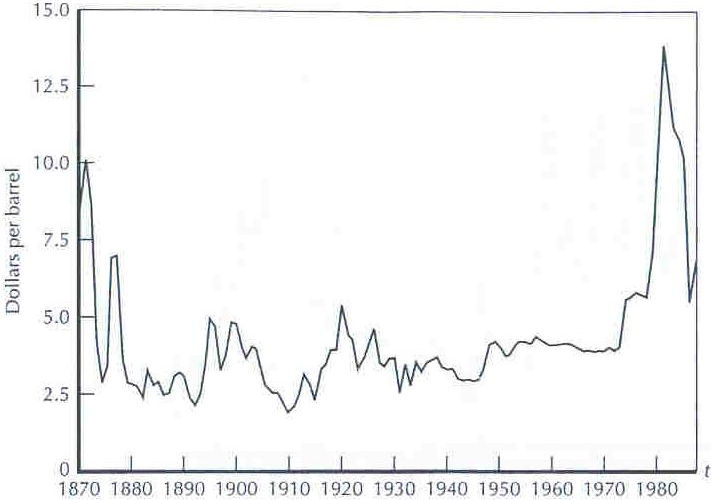
\includegraphics[scale=0.4]{graf1.png}\\   
\textbf{Σχήμα 1.1: Γράφημα χρονοσειράς τιμής αργού πετρελαίου σε δολάρια ανά βαρέλι.}
\end{center} 
\linespread{1}



Η συστηματική μελέτη μιας χρονοσειράς ξεκινάει με την επισκόπηση του
γραφήματός της στο πεδίο του χρόνου, από το οποίο μπορούν αρχικά να ανιχνευθούν
τρία βασικά ποιοτικά χαρακτηριστικά της: Η τάση, η εποχικότητα και οι ακραίες
παρατηρήσεις.\\
\begin{itemize}

\item Η \textbf{τάση} (trend) γενικά θα μπορούσε να ορισθεί ως η μακροπρόθεσμη μεταβολή του
μέσου επιπέδου των τιμών μιας χρονοσειράς. Έτσι, μπορεί η τάση των τιμών να είναι
αυξητική, πτωτική ή σταθερή σε ένα συγκεκριμένο χρονικό διάστημα, ενώ μπορεί και να
έχει τη μορφή κάποιας συνάρτησης στο εν λόγω διάστημα. Να σημειωθεί ότι η έννοια
“μακροπρόθεσμη μεταβολή” εξαρτάται από την εκάστοτε εφαρμογή που εξετάζεται.
\item Η \textbf{εποχικότητα} (seasonal) μπορεί να ορισθεί σαν μια περιοδική διακύμανση που έχει
σταθερό μήκος. Η εν λόγω διακύμανση τις περισσότερες φορές διακρίνεται εύκολα και
μπορεί να ερμηνευθεί στα πλαίσια του υπό μελέτη φαινομένου. Φερ' ειπείν, αν
κανείς επιθυμούσε να αναλύσει τη χρονοσειρά των τιμών των καυσίμων σε βάθος
χρόνων, είναι λογικό να περιμένει να παρατηρήσει μια σχετική άνοδο κατά τους
χειμερινούς μήνες κάθε έτους.

\item Οι \textbf{ακραίες παρατηρήσεις} (outliers) είναι οι απομονωμένες παρατηρήσεις που
εμφανίζονται στο γράφημα κάποιας χρονοσειράς ως απότομες αλλαγές στο πρότυπο
συμπεριφοράς της. Τα outliers μελετήθηκαν αρχικά κατά κύριο λόγο από τον A. J. Fox
(1972), ο οποίος μάλιστα εισήγαγε δύο τύπους. Ο τύπος I αφορά περιπτώσεις όπου η
ύπαρξη μιας ακραίας τιμής δεν έχει καμία επίδραση στις ακόλουθες παρατηρήσεις.
Αντιθέτως, ο τύπος ΙΙ αφορά περιπτώσεις όπου υπάρχει επίδραση στη μετέπειτα
συμπεριφορά των τιμών της χρονοσειράς, παράγοντας μια σειρά λιγότερο ή περισσότερο
ακραίων παρατηρήσεων ή αλλάζοντας εξ’ ολοκλήρου τα χαρακτηριστικά της.
\end{itemize}

%%%%%%%%%%%%%%%%%%%%%%%%%%%%%%%%%%%%%%%%%%
\section{ΣΤΑΤΙΣΤΙΚΑ ΜΕΓΕΘΗ ΧΡΟΝΟΣΕΙΡΩΝ }
%%%%%%%%%%%%%%%%%%%%%%%%%%%%%%%%%%%%%%%%%%
Ως γνωστόν, τα βασικότερα χαρακτηριστικά μιας τυχαίας μεταβλητής $ X $ είναι η
μέση τιμή $\mu = E \left[  X \right]  $, η διασπορά $ \sigma^2 = V \left[  X \right] $ και όταν έχουμε να κάνουμε με ζεύγη
τυχαίων μεταβλητών, η μικτή ροπή 2ας τάξης, δηλαδή η συνδιακύμανση
$\sigma_{xy} = Cov \left(  X , Y \right)  $. Κατ ́ επέκταση, τα βασικότερα χαρακτηριστικά μιας χρονοσειράς
$ \{ X_t : t \in T \}$ είναι:\\
\begin{itemize}
\item H συνάρτηση \textit{μέσης τιμής}
\item Η συνάρτηση \textit{διασποράς}
\item Η συνάρτηση \textit{αυτοσυνδιακύμανσης}

\end{itemize}
\begin{enumerate}


\item \textbf{Η μέση τιμή } ή αναμενόμενη τιμή:\\ $$\quad \mu\left( t  \right) = E\left[ X_t \right], \quad t \in T $$

Στο σημείο αυτό θα πρέπει να αναφέρουμε ότι η μέση τιμή $\mu_t$ σχετίζεται άμεσα
με την έννοια της \textit{τάσης} της χρονοσειράς, εφόσον εκφράζεται ως συνάρτηση της
χρονικής στιγμής $t$ της παρατήρησης $X_t$ . Συγκεκριμένα, αν μια χρονοσειρά παρουσιάζει
αυξητική ή πτωτική τάση αντιστοίχως σε ένα χρονικό διάστημα, αυτό θα αποτυπώνεται
και στη μέση τιμή της $\mu_t$ ως συνάρτηση του χρόνου. Ακόμη, η μη ύπαρξη τάσης σε ένα
χρονικό διάστημα αποτυπώνεται στη σταθερή αναμενόμενη τιμή $\mu_t$ στο εν λόγω
διάστημα.

\item \textbf{Η διασπορά}:\\ $$\sigma^2\left( t \right) =V \left[X_t \right] = E\left[\left( X_t-\mu_t\right) ^2  \right], \quad t \in T    $$

\item \textbf{Η αυτοσυνδιακύμανση}:\\
$$ \gamma\left(t,h \right) = Cov\left(X_t,X_{t+h} \right) =E\left[ \left(X_t-\mu_t \right)\left( X_{t+h}-\mu_{t+h}\right)  \right], \quad t,h \in T   $$ 

Είναι προφανές ότι ισχύει: 
$\sigma^2\left( t \right)=\gamma\left( t,0\right) =Cov\left(X_t,X_t \right),\quad t,h \in T   $ 


\end{enumerate}
%\subsection{ΑΥΤΟΣΥΝΔΙΑΚΥΜΑΝΣΗ}
%\subsection{ ΑΥΤΟΣΥΣΧΕΤΗΣΗ}

%%%%%%%%%%%%%%%%%%%%%%%%%%%%%%%%%%%%%%%%%%%%%
\section{ ΣΤΑΣΙΜΟΤΗΤΑ ΚΑΙ ΑΥΤΟΣΥΣΧΕΤΗΣΗ}
%%%%%%%%%%%%%%%%%%%%%%%%%%%%%%%%%%%%%%%%%%%%%

Είναι φανερό ότι έχοντας παρατηρήσει μια χρονοσειρά
$ \{ X_t : t \in T \} $
από κάποια
χρονική στιγμή $ t = 0 $, έστω μέχρι και την παρούσα χρονική στιγμή $ t = s $, αν δηλαδή
γνωρίζουμε την τροχιά αυτής $ \{ X_t : 0 \leq t \leq s \}$ , και θέλουμε να προβλέψουμε
μελλοντικές τιμές αυτής $ X_{s + h} $, με $ h > 0 $, θα πρέπει να βασιστούμε στις μέχρι τώρα
γνωστές τιμές της και στην εξάρτηση που ενδέχεται να υπάρχει μεταξύ $ X_{s + h} $ και
των τιμών
$ \{ X_t : 0 \leq t \leq s \}$
της χρονοσειράς στο παρελθόν. Τούτο βέβαια με την
προϋπόθεση ότι όλα τα πιθανοθεωρητικά χαρακτηριστικά μιας χρονοσειράς, ή
τουλάχιστον τα βασικότερα εξ αυτών, παραμένουν αναλλοίωτα στον χρόνο. \\ \\
Όταν όλα τα πιθανοθεωρητικά χαρακτηριστικά μιας χρονοσειράς παραμένουν
αναλλοίωτα στο χρόνο τότε μιλάμε για \textit{αυστηρή στασιμότητα}. Συγκεκριμένα έχουμε:
\begin{enumerate}
\item \textbf{ Αυστηρή Στασιμότητα} \\\\
Η χρονοσειρά $\: \{ X_t: t \in T \} \: $ ονομάζεται
\textit{αυστηρά στάσιμη} όταν $ \forall n \in N,\:  t_i \in T $ με $ i=1,\ldots ,n $  και  $ h \in T $
ισχύει η παρακάτω
σχέση ισοδυναμίας \\
$$ \left( X_{t_1}, \ldots , X_{t_n} \right)  \sim \left( X_{t_1+h}, \ldots , X_{t_n+h}    \right) $$


Εδώ το σύμβολο “ $\sim$ ” διαβάζεται “κατανέμεται όπως”, ή “ισοκατανέμεται με”. \\\\
Συνεπώς οι κατανομές πεπερασμένης διάστασης αυστηρώς στάσιμων
χρονοσειρών παραμένουν αναλλοίωτες σε χρονικές μεταθέσεις. 

\item \textbf{ Ασθενής Στασιμότητα} \\\\
Η χρονοσειρά
$ \{ X_t : t \in T \}$
ονομάζεται
\textit{ασθενώς στάσιμη}, ή υπό ευρεία έννοια, στάσιμη όταν οι ροπές πρώτης και δεύτερης τάξης είναι σταθερές στo
χρόνο, δηλαδή: \\
\begin{itemize}
\item Η μέση τιμή είναι σταθερή: $  \mu = E \left[ X_t \right] ,\quad t \in T $
\item $ \gamma(h)=Cov(X_t,X_{t+h}), \quad t,h \in T $
\end{itemize} 
\end{enumerate}

H συνάρτηση \textit{αυτοσυσχέτισης} στάσιμης χρονοσειράς ορίζεται από τη
σχέση:\\
$$ \rho\left(h \right)=Corr\left( X_0,X_h\right) =\frac{Cov\left( X_0,X_h\right) }{\sqrt{V\left[X_0 \right]V\left[ X_h\right]  }}=\frac{\gamma\left(h \right) }{\gamma\left(0 \right) }, \quad h \in T  $$



%\section{ΕΡΓΟΔΙΚΟΤΗΤΑ}
%\section{ΠΡΩΤΑ ΣΤΑΔΙΑ ΑΝΑΛΥΣΗΣ}










%%%%%%%%%%%%%%% File ends here %%%%%%%%%%%%%%%%%%%%%%%%%%%%%%%%
\endinput
%%% Local Variables: 
%%% mode: latex
%%% TeX-master: "ptyxiakn"
%%% End: 
